\sourcepage{1}
\hypersetup{pageanchor=false}
\begin{titlepage}
\centering
\vspace*{25mm}
{\Huge\bfseries\heiti\color{dcrteal}临床研究设计\par}
\vspace{8mm}
{\LARGE Designing Clinical Research\par}
\vspace{7mm}
{\Large 第五版\par}
\vspace{18mm}
{\large Warren S. Browner\quad Thomas B. Newman\par
Steven R. Cummings\quad Deborah G. Grady\par
Alison J. Huang\quad Alka M. Kanaya\quad Mark J. Pletcher\par}
\vfill
{\large Wolters Kluwer\par}
\vspace{8mm}
{\small 中文译本\quad 底本版权年份：2023\par}
\end{titlepage}
\hypersetup{pageanchor=true}
\sourcepage{3}
\chapter*{作者}
\addcontentsline{toc}{chapter}{作者}
\begingroup\small
\noindent\textbf{Warren S. Browner, MD, MPH}\\
Sutter Health California Pacific Medical Center 首席执行官；加利福尼亚大学旧金山分校流行病学与生物统计学临床教授。

\noindent\textbf{Thomas B. Newman, MD, MPH}\\
加利福尼亚大学旧金山分校流行病学与生物统计学、儿科学荣休教授。

\noindent\textbf{Steven R. Cummings, MD}\\
California Pacific Medical Center Research Institute 下属 San Francisco Coordinating Center 执行主任；加利福尼亚大学旧金山分校医学、流行病学与生物统计学荣休教授。

\noindent\textbf{Deborah G. Grady, MD, MPH}\\
\textit{JAMA Internal Medicine} 副主编；加利福尼亚大学旧金山分校医学、流行病学与生物统计学荣休教授。

\noindent\textbf{Alison J. Huang, MD, MAS}\\
加利福尼亚大学旧金山分校医学、泌尿学、流行病学与生物统计学教授。

\noindent\textbf{Alka M. Kanaya, MD}\\
加利福尼亚大学旧金山分校医学、流行病学与生物统计学教授。

\noindent\textbf{Mark J. Pletcher, MD, MPH}\\
加利福尼亚大学旧金山分校流行病学与生物统计学、医学教授。
\endgroup

\sourcepage{4}
\chapter*{出版信息}
\begingroup\fontsize{9.5}{14}\selectfont
\noindent 选题编辑：Joe Cho\\
开发编辑：Ariel S. Winter\\
编辑协调：Sean Hanrahan\\
编辑助理：Maribeth Wood\\
营销经理：Kristen Watrud\\
制作项目经理：David Saltzberg\\
设计协调：Steve Druding\\
生产协调：Beth Welsh\\
印前服务：S4Carlisle Publishing Services

第五版。版权所有 \copyright\ 2023 Wolters Kluwer。

版权所有 \copyright\ 2013 LIPPINCOTT WILLIAMS \& WILKINS（WOLTERS KLUWER 旗下企业）；\copyright\ 2007 Lippincott Williams \& Wilkins（Wolters Kluwer 旗下企业）；2001 Lippincott Williams \& Wilkins；1998 Williams \& Wilkins。保留所有权利。本书受版权保护。未经版权所有者书面许可，不得以任何形式或方式复制、传播本书的任何部分，包括影印、扫描或其他电子复制，也不得利用任何信息存储与检索系统使用本书；评论文章及书评中的简短引文除外。美国政府雇员在履行公务时编写并收入本书的材料不受上述版权声明约束。申请许可，请联系 Wolters Kluwer，地址为 Two Commerce Square, 2001 Market Street, Philadelphia, PA 19103；电子邮箱为 \href{mailto:permissions@lww.com}{permissions@lww.com}，或访问网站 \url{https://shop.lww.com}（产品与服务）。

\noindent 9 8 7 6 5 4 3 2 1\\在新加坡印刷。

\noindent\textbf{美国国会图书馆出版物编目数据}

姓名：Browner, Warren S.，作者。\\
书名：Designing clinical research / Warren S. Browner, Thomas B. Newman, Steven R. Cummings, Deborah G. Grady, Alison J. Huang, Alka M. Kanaya, Mark J. Pletcher。\\
描述：第五版。Philadelphia: Wolters Kluwer Health, [2023]。
\sourcepage{5}
前版：Designing clinical research / Stephen B. Hulley … [et al.]，第四版，2013 年。含参考文献与索引。\\
标识符：LCCN 2021043257（印刷本）；LCCN 2021043258（电子书）；ISBN 9781975174408（平装）；ISBN 9781975174422（电子书）。\\
主题：MESH: Epidemiologic Methods（流行病学方法）；Research Design（研究设计）。\\
分类：LCC RA651（印刷本）；LCC RA651（电子书）；NLM WA 950；DDC 614.4072—dc23。\\
国会图书馆印刷本记录：\url{https://lccn.loc.gov/2021043257}。\\
电子书记录：\url{https://lccn.loc.gov/2021043258}。

本书按“现状”提供。出版者不作任何明示或默示担保，包括对内容准确性、全面性或时效性的担保。

本书不能代替医疗专业人员对具体患者进行评估；这种评估应依据对每位患者的检查，并考虑其年龄、体重、性别、目前及既往疾病、用药史、实验室数据以及患者特有的其他因素。出版者不提供医疗建议或指导，本书仅为参考工具。使用本书的一切责任，包括所有医学判断及由此产生的诊断与治疗，均由医疗专业人员承担，出版者不承担这些责任。

鉴于医学科学和健康信息持续快速发展，对医学诊断、适应证、适当的药物选择与剂量及治疗方案，应进行独立的专业核实，医疗专业人员也应参考多种来源。处方用药时，建议查阅每种药品随附的产品资料（生产商的药品说明书），核实使用条件、警告、不良反应等，并确认给药方案或禁忌证是否有变化；对新药、不常使用的药物或治疗窗狭窄的药物尤须如此。在适用法律允许的最大范围内，出版者不对任何人因参考或使用本书而遭受的人身伤害和／或财产损失承担责任，无论该责任涉及产品责任、过失法或其他法律依据。

\noindent\url{https://shop.lww.com}
\endgroup

\sourcepage{6}
\chapter*{献辞}
\begin{center}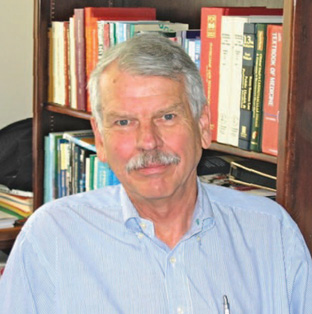
\includegraphics[width=52mm]{assets/stephen_hulley.jpeg}\end{center}
献给 Stephen Hulley, MD, MPH。他构思、孕育并悉心培育了本书前四版；层层修订之下，他留下的文字与思想依然熠熠生辉。

献给我们的家人，感谢他们包容我们对深奥概念的执着，以及迫近截稿日期时的忙碌。

也献给我们的老师、同事与学生，感谢他们激励我们钻研得更深、讲解得更好。

\sourcepage{9}
\chapter*{撰稿作者}
\addcontentsline{toc}{chapter}{撰稿作者}
\noindent\textbf{Daniel Dohan, PhD}\\
加利福尼亚大学旧金山分校 Philip R. Lee 卫生政策研究所教授。

\noindent\textbf{Michael A. Kohn, MD, MPP}\\
加利福尼亚大学旧金山分校流行病学与生物统计学荣休教授。

\noindent\textbf{Bernard Lo, MD}\\
加利福尼亚大学旧金山分校医学荣休教授、医学伦理项目荣休主任。

\sourcepage{10}
\chapter*{引言}
\addcontentsline{toc}{chapter}{引言}
《临床研究设计》（\textit{Designing Clinical Research}，DCR）第五版问世，恰逢本书初版出版 35 周年。这也是第一部没有由我们无畏的导师 Steve Hulley 主持编写的版本，后文还会谈到他。本书最初只是一次小型研讨课的讲义汇编，如今已成为本领域使用最广泛的教材，累计销量超过 15 万册。

DCR 自始面向处于职业起步阶段的临床研究者。他们可能在求学过程中上过流行病学（epidemiology）课程，还记得其中一些概念，但更可能已经不记得了。事实上，我们中的许多人（SRC、WSB、TBN 和 DGG）四十年前开始学术生涯时，也是类似情形：我们对临床研究感兴趣，在培训期间参加过讨论并批评已发表论文的文献研读会，却对如何设计一项研究毫无头绪。当时，多数学术医疗中心在这方面能提供的帮助很少。

幸而 Steve Hulley 意识到，虽然流行病学是临床研究的基础科学，许多研究的设计者和负责人却几乎没有流行病学训练与认识。当时，对基础研究感兴趣的专科进修医师，在实验台前开始项目之前，会接受实验技术培训；而对临床研究感兴趣的人，大多只能自行摸索，有时甚至被建议选择更传统的职业道路。Steve 填补了这个空白：先开设并讲授如何设计临床研究的课程，再主持由 Andrew W. Mellon Foundation 资助的进修项目，培养一批“临床流行病学家”（我们这个新专科甚至配有黄铜名牌），最后在我们这些刚受训的门生展翅起飞时继续给予指导。所有这些都发生在加利福尼亚大学旧金山分校（University of California, San Francisco，UCSF）——这所健康科学大学，\sourcepage{11}无论当时还是现在，都以对基础研究的投入和成就最为人熟知。

从一开始，DCR 就代表着 Steve 愿景的下一步：让这些知识走出旧金山湾区。如今，许多读者是世界各地刚开始从事临床研究、或至少正在考虑这条道路的健康科学学生与从业者。本书已有阿拉伯文、中文、日文、韩文、西班牙文和葡萄牙文译本。他们逐渐认识到，设计能够为循证临床实践提供信息的研究，需要作出许多判断，而流行病学原理可以指导这些判断。

第五版仍忠于作为入门教材而非百科全书的初衷，同时更新了我们理解因果效应（causal effects）的方式——有人也许会说：“总算更新了！”为反映流行病学家思维方式的发展，我们新增了反事实模型（counterfactual models）和有向无环图（directed acyclic graphs）的介绍。多年来，我们一直没有作这项改变，因为这部分位于全书中心的内容，在理解上颇具挑战。我们希望读者沿着长长的栈桥走入水中之后，会觉得这趟游泳值得：对流行病学家如何估计因果效应，有了更深的理解。

我们新增了社区参与式研究（community-engaged research）和定性研究（qualitative studies）两章，反映这些方法在临床研究中日益重要的地位。我们把习题移到各章末尾，希望它们更容易被注意到，而答案仍留在书末。术语释义已经扩充，正文中用红色标出在其中定义的概念。几乎所有插图都重新设计，并用一致的颜色表示研究设计的不同方面，例如靛蓝色表示干预，紫色表示预测变量，赭黄色表示结局。更重要的是，我们邀请了三位“年轻”作者参与——他们每一位的资历，都比其余作者当年开始编写第一版时更深。这在一定程度上反映了临床研究自 1988 年以来的巨大增长：接受过良好训练的临床研究者更多了，\sourcepage{12}他们也已在学术界逐步晋升。我们希望后续版本也能有类似的新鲜血液。

第五版配有 DCR 网站 \url{https://dcr-5.net}，提供教学材料，包括我们每年在 UCSF 为学员开设的 4 周及 7 周 DCR 工作坊的详细课程大纲链接。此外，网站也为研究者提供实用工具，其中包括出色的交互式样本量（sample size）计算器 \url{https://www.sample-size.net}。

本书也有许多未变之处。正如 Steve Hulley 的初衷，第五版仍明确面向职业起步阶段的临床研究者。我们尽量避免行话和技术术语，聚焦重要问题，例如怎样找到好的研究问题，以及怎样形成高效、有效且符合伦理的研究设计。譬如，样本量估算两章使没有统计学训练的读者，也能自行完成计算，无须与公式搏斗。因果推理部分用简单的例子与图形讲解复杂主题。我们仍在第一分部使用女性代词、第二分部使用男性代词，并在最后一分部改用复数代词，以鼓励所有临床研究者。不过，DCR 仍未讨论如何分析、呈现和发表临床研究结果等重要领域；读者可以通过其他书籍继续学习这些主题（1—4）。

最后，提出几点建议。要成为独立的临床研究者，必须跨越两道障碍：成为一篇重要论文的第一作者，以及成为一项经过同行评议资助项目的主要研究者。本书可以帮助你实现这些目标，尤其是在另一个必要条件的配合下：有一位关心你和你职业发展的研究导师。我们强烈建议，你在购买或借阅本书之后，找一位资深同事，在设计与执行临床研究项目的复杂过程中给予支持。

获得培训的机会增多了，竞争也更加激烈，达到独立开展研究所需的时间也更长。坚持与创造力同样重要。我们每个人都收到过不计其数的期刊与资助机构拒信。\sourcepage{13}得知自己的工作和想法有价值、却还不够出色或还不到时候，难免令人气馁。有时似乎许多最有意思的问题都已得到回答，但那只是错觉。可预防的疾病仍然经常发生，另一些疾病如何预防还不得而知。潜在的治疗方法和创新诊断试验每天都在开发。大量人群及其健康相关关切，在研究中一直系统性地缺少代表。有这么多机会，追求真理与公正完全可以成为毕生事业。

\begin{references}
\item Vittinghoff E, Glidden DV, Shiboski SC, et al. \textit{Regression Methods in Biostatistics: Linear, Logistic, Survival, and Repeated Measures Models}. 2nd ed. Springer-Verlag; 2012.
\item Katz MH. \textit{Multivariable Analysis: A Practical Guide for Clinicians and Public Health Researchers}. 3rd ed. Cambridge University Press; 2011.
\item Newman TB, Kohn MA. \textit{Evidence-Based Diagnosis: An Introduction to Clinical Epidemiology}. 2nd ed. Cambridge University Press; 2020.
\item Browner WS. \textit{Publishing and Presenting Clinical Research}. 3rd ed. Lippincott Williams \& Wilkins; 2012.
\end{references}

\sourcepage{14}
\chapter*{致谢}
\addcontentsline{toc}{chapter}{致谢}
感谢加利福尼亚大学旧金山分校，特别是流行病学与生物统计学系，在过去四十年中为我们提供了滋养成长的家园；感谢 UCSF、California Pacific Medical Center Research Institute 及世界各地从事临床研究的同事；也感谢 Wolters Kluwer 团队帮助我们完成新版。特别感谢 Anita Stewart 在自报测量方面提供帮助，Frank Harrell 启发我们加入贝叶斯方法（Bayesian approaches），以及 John Boscardin 和 Martina Steurer 协助制作部分插图。

我们也感谢那些致力于改善世界的同事。为表达谢意，本书的部分版税将捐赠给推动地区或全球健康的组织，包括社会责任医师协会（Physicians for Social Responsibility，\url{https://www.psr.org}）、Americares（\url{https://www.americares.org}）和 Institute on Aging（\url{https://ioaging.org}）。
